% Local numeric construction, not source data. Replace every object.
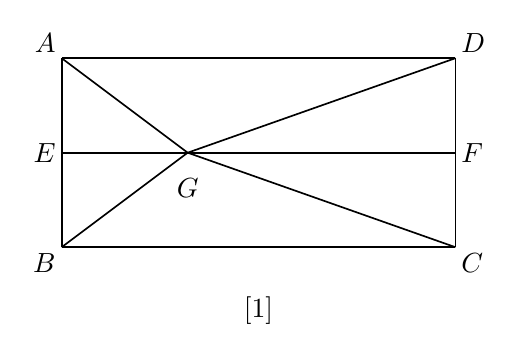
\begin{tikzpicture}[x=1cm,y=1cm,font=\normalsize,
 geometry edge/.style={solid,line width=.6pt},
 geometry mark/.style={solid,line width=.6pt},
 geometry label/.style={font=\normalsize,inner sep=2pt}]
\coordinate (A) at (0,2.4);
\coordinate (B) at (0,0);
\coordinate (C) at (5.000000000,0.000000000);
\coordinate (D) at (5.000000000,2.400000000);
\coordinate (E) at (0,1.2);
\coordinate (F) at (5.000000000,1.200000000);
\coordinate (G) at (1.600000000,1.200000000);
\draw[geometry edge] (A)--(B);
\draw[geometry edge] (B)--(C);
\draw[geometry edge] (C)--(D);
\draw[geometry edge] (D)--(A);
\draw[geometry edge] (E)--(G);
\draw[geometry edge] (G)--(F);
\draw[geometry edge] (A)--(G);
\draw[geometry edge] (G)--(C);
\draw[geometry edge] (B)--(G);
\draw[geometry edge] (G)--(D);
\node[geometry label,above left] at (A) {$A$};
\node[geometry label,below left] at (B) {$B$};
\node[geometry label,below right] at (C) {$C$};
\node[geometry label,above right] at (D) {$D$};
\node[geometry label,left] at (E) {$E$};
\node[geometry label,right] at (F) {$F$};
\node[geometry label,below,yshift=-7pt] at (G) {$G$};
\node[font=\normalsize] at (2.5,-.8) {\bitmapinsertcaption[1]};
\end{tikzpicture}
